\documentclass[
11pt, % The default document font size, options: 10pt, 11pt, 12pt
oneside, % Two side (alternating margins) for binding by default, uncomment to switch to one side
italian, %english, % ngerman for German
onehalfspacing,%singlespacing, % Single line spacing, alternatives: onehalfspacing or doublespacing
%draft, % Uncomment to enable draft mode (no pictures, no links, overfull hboxes indicated)
%nolistspacing, % If the document is onehalfspacing or doublespacing, uncomment this to set spacing in lists to single
%liststotoc, % Uncomment to add the list of figures/tables/etc to the table of contents
%toctotoc, % Uncomment to add the main table of contents to the table of contents
%parskip, % Uncomment to add space between paragraphs
%nohyperref, % Uncomment to not load the hyperref package
headsepline, % Uncomment to get a line under the header
%twocolumn,
% chapterinoneline, % Uncomment to place the chapter title next to the number on one line
%consistentlayout, % Uncomment to change the layout of the declaration, abstract and acknowledgements pages to match the default layout
]{MastersDoctoralThesis} % The class file specifying the document structure

\usepackage[utf8]{inputenc} % Required for inputting international characters
\usepackage[T1]{fontenc} % Output font encoding for international characters
%\usepackage{mathpazo} % Use the Palatino font by default
\usepackage[backend=bibtex, sorting=none, natbib=true]{biblatex} % Use the bibtex backend with the authoryear citation style (which resembles APA)
\usepackage[autostyle=true]{csquotes} % Required to generate language-dependent quotes in the bibliography
\usepackage{enumitem}
\usepackage{listings}
\usepackage{graphicx}
\usepackage{xcolor}
\usepackage{amsmath}
\usepackage[font={small}]{caption}
\usepackage{varwidth}
\usepackage{supertabular}
\usepackage[caption=false]{subfig}
\usepackage{wrapfig}
\usepackage{mathtools}
\usepackage{titlesec}
\usepackage{hyperref}

\newcommand\citen[1]{\citeauthor{#1} \citep{#1}}
\newcommand\citetitlen[1]{\citetitle{#1} \citep{#1}}
\addbibresource{related_work.bib} % The filename of the bibliography

\graphicspath{
    {Figures/}{images/}
}

\newenvironment{blueparagraph}{\par\color{blue}}{\par}
\newenvironment{nscenter}
 {\parskip=0pt\par\nopagebreak\centering}
 {\par\noindent\ignorespacesafterend}

 \titleformat{\chapter}[display]
 {\normalfont\bfseries}{}{0pt}{\huge}

%----------------------------------------------------------------------------------------
%	MARGIN SETTINGS
%----------------------------------------------------------------------------------------

\geometry{
	paper=a4paper, % Change to letterpaper for US letter
	inner=2.5cm, % Inner margin
	outer=3.8cm, % Outer margin
	bindingoffset=.5cm, % Binding offset
	top=1.5cm, % Top margin
	bottom=1.5cm, % Bottom margin
	%showframe, % Uncomment to show how the type block is set on the page
}

\usepackage{graphicx}
\usepackage{multicol}

\setlength{\columnsep}{0.3in}

\pdfpagewidth 8.5in
\pdfpageheight 11in

\setlength{\textwidth}{6.5in}
\setlength{\oddsidemargin}{0.0in}
\setlength{\evensidemargin}{0.0in}
\setlength{\textheight}{9in}
\setlength{\topmargin}{-36pt}
\setlength{\headheight}{12pt}
\setlength{\headsep}{24pt}
\setlength{\footskip}{24pt}
\setlength{\parskip}{4pt plus 1pt}
\renewcommand{\baselinestretch}{1.125} %1.0

\pagenumbering{arabic}

%   PUNCTUATION SPACING
%  By default, punctuation [.?!:;,] is followed by extra space EXCEPT
%  when the punctuation follows an upper case letter.  The following
%  removes the exception, i.e., punctuation will produce extra space
%  regardless of what character precedes the punctuation.  If you
%  don't want the extra space, follow the offending punctuation mark
%  with '\ ' or '~'.  \frenchspacing and \nonfrenchspacing work as
%  usual to turn extra spacing off and back on, respectively.

\sfcode`A=1000 \sfcode`B=1000 \sfcode`C=1000 \sfcode`D=1000
\sfcode`E=1000 \sfcode`F=1000 \sfcode`G=1000 \sfcode`H=1000
\sfcode`I=1000 \sfcode`J=1000 \sfcode`K=1000 \sfcode`L=1000
\sfcode`M=1000 \sfcode`N=1000 \sfcode`O=1000 \sfcode`P=1000
\sfcode`Q=1000 \sfcode`R=1000 \sfcode`S=1000 \sfcode`T=1000
\sfcode`U=1000 \sfcode`V=1000 \sfcode`W=1000 \sfcode`X=1000
\sfcode`Y=1000 \sfcode`Z=100


%----------------------------------------------------------------------------------------
%	THESIS INFORMATION
%----------------------------------------------------------------------------------------

\thesistitle{Attacco e difesa di Cryptojacking basato su GPU} % Your thesis title, this is used in the title and abstract, print it elsewhere with \ttitle
%\supervisor{Dr.\ Name \textsc{Surname}} % Your supervisor's name, this is used in the title page, print it elsewhere with \supname
%\examiner{} % Your examiner's name, this is not currently used anywhere in the template, print it elsewhere with \examname
%\degree{Computer Science} % Your degree name, this is used in the title page and abstract, print it elsewhere with \degreename
\author{Federico \textsc{Zappone}} % Your name, this is used in the title page and abstract, print it elsewhere with \authorname
%\addresses{} % Your address, this is not currently used anywhere in the template, print it elsewhere with \addressname

\subject{Networking security and software security} % Your subject area, this is not currently used anywhere in the template, print it elsewhere with \subjectname
\keywords{GPU, cryptojacking, xss, defence} % Keywords for your thesis, this is not currently used anywhere in the template, print it elsewhere with \keywordnames
\university{\href{https://www.unimol.it/}{Università del Molise}} % Your university's name and URL, this is used in the title page and abstract, print it elsewhere with \univname
\department{\href{http://dipbioter.unimol.it/}{Dipartimento di Bioscienze e Territorio}} % Your department's name and URL, this is used in the title page and abstract, print it elsewhere with \deptname
%\faculty{\href{http://faculty.university.com}{Faculty Name}} % Your faculty's name and URL, this is used in the title page and abstract, print it elsewhere with \facname

\AtBeginDocument{
\hypersetup{pdftitle=Title\ttitle} % Set the PDF's title to your title
\hypersetup{pdfauthor=Federico Zappone\authorname} % Set the PDF's author to your name
\hypersetup{pdfkeywords=keyword1 keyword2 keyword3 \keywordnames} % Set the PDF's keywords to your keywords
}

\begin{document}
\renewenvironment{abstract}

%\frontmatter % Use roman page numbering style (i, ii, iii, iv...) for the pre-content pages

\pagestyle{plain} % Default to the plain heading style until the thesis style is called for the body content

%----------------------------------------------------------------------------------------
%	TITLE PAGE
%----------------------------------------------------------------------------------------

\begin{titlepage}
\begin{center}

\vspace*{.06\textheight}
{\scshape\LARGE \univname\par}\vspace{0.5cm} % University name
{\scshape\large \deptname\par}\vspace{1cm} % University name


\includegraphics[width=0.25\textwidth]{images/logo.png} % University/department logo - uncomment to place it
\vspace{1cm}

\textsc{\Large Proposta di progetto}\\[0.5cm] % Thesis type

\HRule\\[0.4cm] % Horizontal line
{\huge \bfseries \ttitle\par}\vspace{0.4cm} % Thesis title
\HRule\\[1.5cm] % Horizontal line

%\begin{minipage}[t]{0.4\textwidth}
\begin{center} \large
\emph{Author:}\\
\href{mailto:f.zappone1@studenti.unimol.it}{\authorname} % Author name - remove the \href bracket to remove the link
\end{center}
%\end{minipage}
%\begin{minipage}[t]{0.4\textwidth}
%\begin{flushright} \large
%\emph{Supervisor:} \\
%\href{Supervisor ref}{\supname} % Supervisor name - remove the \href bracket to remove the link
%\end{flushright}
%\begin{flushright} \large
%\emph{Correlator:} \\
%\href{Correlator ref}{Name Surname} % Correlator name
%\end{flushright}
%\end{minipage}\\[3cm]

%\vfill

\centerline{\large \subjectname}
%\bigskip
{\large Dicembre 01, 2020}\\[2cm] % Date
\vfill
\end{center}
\end{titlepage}

%----------------------------------------------------------------------------------------
%	QUOTATION PAGE
%----------------------------------------------------------------------------------------

%\vspace*{0.2\textheight}

%\noindent\enquote{\itshape Thanks to my solid academic training, today I can write hundreds of words on virtually any topic without possessing a shred of information, which is how I got a good job in journalism.}\bigbreak

%\hfill Dave Barry


%----------------------------------------------------------------------------------------
%	ABSTRACT PAGE
%----------------------------------------------------------------------------------------

% \begin{abstract}
%   \chapter*{Abstract}

% \end{abstract}

% \vspace*{50px}
% \bigskip

%----------------------------------------------------------------------------------------
%	TABLE OF CONTENTS AND LIST OF FIGURES
%----------------------------------------------------------------------------------------

%\tableofcontents
%\newpage

%\listoffigures
%\newpage

%----------------------------------------------------------------------------------------
%	PROPOSAL
%----------------------------------------------------------------------------------------

{\chapter{Introduzione}}
In quest'ultimo decennio si è molto discusso di monete digitali e delle così dette criptovalute in seguito all'avvento delle blockchain. Quest'ultima è una tecnologia basata sul concetto di database distribuito, ovvero un sistema che utilizza un registro condiviso per salvare informazioni, esso è accessibile solo ai nodi della stessa rete ed è rappresentabile come una successione di blocchi contenenti le informazioni. Contemporaneamente alle blockchain è nata anche la prima criptovaluta, più precisamente, il 3 gennaio 2009 veniva scritto il primo blocco di \emph{Bitcoin}~\citep{kharraz2019outguard} dal valore complessivo inferiore a un dollaro statunitense. In seguito il 6 novembre 2010 \emph{Bitcoin} si presentava con un valore di \$0,50, in meno di due anni il prezzo era aumentato di 625 volte, e da allora in poco più di sette anni, raggiunse il suo massimo storico di quasi \$20.000 ovvero circa 40.000 volte in più~\citep{bitcoinwiki}~\citep{wiredbitcoin}. Divenuto un caso più unico che raro, \emph{Bitcoin} si è posto da apripista a più di 5000 altre criptovalute~\citep{coinlore} fino ad essere definito come l'oro del \RN{21} secolo. Questa definizione non è dovuta solo all'incredibile aumento del prezzo negli ultimi anni ma anche ad una delle caratteristiche chiave che sia l'oro che la maggior parte delle criptovalute condivide, il processo di ``estrazione'' definito appunto come \emph{mining} nel campo delle monete digitali.\\
Il \emph{mining} di criptovalute consiste nel creare monete virtuali attraverso la risoluzione di alcune funzioni crittografiche necessarie per la validazione delle transazioni e dei blocchi che compongono una blockchain. Questa operazione termina con un compenso da parte della blockchain al \emph{miner}, il quale, avendo offerto la sua potenza di calcolo viene premiato con la stessa criptovaluta minata. Questi calcoli vengono eseguiti da sistemi informatici dedicati a questo specifico processo, essi sono divisi in due grandi macro sezioni: quelli che sfruttano la Central Processing Unit (CPU) e quelli che sfruttano la Graphics processing unit (GPU). I primi prendono il nome di \emph{ASIC}, acronimo di \emph{Application Specific Integrated Circuit}, ovvero circuiti costruiti per la risoluzione di un calcolo ben specifico che risultano però molto inefficienti su altri tipi di algoritmi. I sistemi basati su GPU sono invece spesso molto più prestanti, le schede video riescono infatti a effettuare più calcoli al secondo rispetto alle CPU che risultano quindi meno redditizie nella maggior parte dei casi di \emph{mining}. D'altro canto per le GPU risulta essere molto più difficile la gestione delle temperature e inoltre comportano costi maggiori sia in termini di assemblaggio che di costi energetici per il mantenimento. Proprio questi ultimi aspetti sono quelli di notevole impatto per il \emph{mining}: il costo di acquisto delle componenti è nettamente aumentato negli ultimi anni, questo sia a causa delle nuove scoperte tecnologiche più performanti, sia a causa delle grandi farm di \emph{mining} che costantemente acquistano nuove schede video.\\
Con l'aumentare dei costi di \emph{mining}, e allo stesso tempo delle opportunità di guadagno offerte dal mondo in crescita delle blockchain, le criptovalute hanno iniziato a risaltare agli occhi del crimine informatico. Più precisamente la tecnologia blockchain, e di conseguenza le criptovalute, posseggono, per lo meno la maggior parte di esse, una caratteristica molto importante per i cyber criminali, ovvero garantiscono una certa forma di anonimato. Le criptovalute infatti non sono in alcun modo collegabili a un individuo diversamente da un conto bancario, l'unico ad averne pieno controllo è colui che le possiede. Questa caratteristica ha portato a un enorme utilizzo delle criptovalute per lo svolgimento di azioni illecite, nel 2017 infatti si è riscontrato un netto aumento di \emph{ransomware}~\citep{skyboxtrends}, ovvero quei virus che una volta bloccato il sistema al quale accedono chiedono un riscatto per il suo sblocco. L'incremento di questi attacchi è dovuto principalmente alla pratica dei cyber criminali di richiedere il riscatto sotto forma di criptovalute per mantenere l'anonimato. Successivamente si è arrivati a una forma di attacco più intelligente e meno invasiva che utilizza i \emph{cryptominers}. Definito appunto come ``l'anno dei cryptominers'', il 2018 vede la stessa impennata di casi di \emph{ransomware} dell'anno precedente sotto una nuova forma di attacco che si appropria di criptovalute in modo illegale ma sfruttando un'operazione lecita come quella del \emph{mining}~\ref{fig:topmalwarefamilies}. Questa tecnica detta \emph{cryptojacking} consiste in programmi che utilizzano il computer della vittima per l'estrazione di criptovalute ma, diversamente dal \emph{mining} legittimo, il guadagno di questo processo viene poi attribuito non ai possessori del calcolatore bensì all'attaccante. Il tutto avviene seguendo un basso profilo, tramite programmi infetti che vengono installati sul computer o, come più recentemente si è affermato, utilizzando script malevoli presenti all'interno di pagine web. La sostanziale differenza tra le tecniche sta principalmente nella loro rintracciabilità, infatti quelli che operano attraverso il web sono più difficili da individuare e analizzare rispetto a programmi che vengono installati e che sono quindi sotto l'occhio diretto di antivirus e delle politiche dettate dal sistema operativo.\\
Le GPU grazie alla loro potenza offrono quindi nella maggior parte dei casi dei ricavi maggiori nel \emph{mining} rispetto alle CPU, di contro però non sono facilmente utilizzabili in ambito web. Ciò ha portato infatti ad uno sviluppo maggiore dei \emph{cryptominers} basati su CPU e, di conseguenza, a sistemi di difesa che si concentrano su di essi, trascurando le minacce derivanti da attacchi pensati per Graphics Processing Unit. Infatti sia \citen{musch2018web} che \citen{saad2018end} mostrano la diffusione di \emph{cryptominers} basati su CPU nei siti web, inoltre analizzano l'efficacia di tecniche difensive di blacklisting che risultano però essere una protezione insufficiente e poco pratica. \citen{wang2018seismic} forniscono in seguito un metodo di analisi di firme basate su istruzioni della CPU durante l'esecuzione dei moduli \emph{WebAssembly}. \citen{konoth2018minesweeper} introducono invece \emph{MineSweeper} basato anch'esso sul precedente principio di firme ma aggiunge inoltre il rilevamento di eccessive chiamate di sistema di natura crittografica durante l'esecuzione di un programma. \citen{kharraz2019outguard} dimostrano invece che come l'analisi della CPU generi una grande quantità di falsi positivi all'interno della navigazione web. Un differente approccio viene fornito da \citen{tahir2017mining} che presentano \emph{MineGuard}, un sistema che tramite l'analisi delle prestazioni hardware rileva l'esecuzione di alcuni algoritmi di \emph{mining}. \emph{MineGuard} monitora costantemente sia CPU che GPU ed inoltre offre un'ottima soluzione sia in termini di efficienza che di utilizzo di risorse per la sua esecuzione. \citen{belkin2019risks} offrono infine una soluzione dedicata esclusivamente a \emph{cryptominers} di GPU che risulta essere più pratica in ambito web rispetto alle altre, questo analizzando le pagine web che utilizzano \citetitlen{WebGL}. Quest'ultima è una delle librerie web basate sulla specifica \citetitle{OpenGL} (\emph{Open Graphics Library}) considerata ormai lo standard per quanto riguarda la grafica tridimensionale in sistemi operativi \emph{Unix-like}. In particolare \citetitle{OpenGL} è stata pensata per architetture parallelizzabili come le GPU e definisce delle \emph{API} per applicazioni che operano in ambienti 3D.\ Su questo standard sono basate le librerie che permettono di utilizzare la GPU in ambito web. Più precisamente \citetitle{WebGL} è una \emph{Web-based Graphics Library} ovvero una libreria pensata per la gestione di elementi grafici all'interno del web, essa fornisce delle \emph{API} per grafica 3D in un contesto \emph{HTML5} tramite l'utilizzo del \emph{Document Object Model (DOM)}. \citetitle{GPU.js} è invece una libreria scritta interamente in \emph{JavaScript}, pensata per sfruttare l'accelerazione hardware delle GPU basata a sua volta su \citetitle{WebGL}.\\
L'idea di base di questo progetto è quindi quella di sviluppare un \emph{cryptominer} che, attraverso lo standard \citetitlen{OpenGL} e l'utilizzo di un linguaggio di scripting, sia in grado di effettuare \emph{mining} di criptovalute sfruttando la GPU.\ L'utilizzo di un linguaggio di scripting web è necessario visto che per portare a termine l'attacco saranno sfruttate le vulnerabilità al \emph{Cross Site Script (XSS)}. Gli attacchi di tipo \emph{XSS} sono tra i più diffusi nel web, infatti, secondo il report di \citen{PositiveTechnologiesReport}, la percentuale di questi attacchi è salita dall'occupare il 77,9\% nel 2017 all'88,5\% di tutte le tipologie di attacchi web registrate nel 2018. Secondo \citen{PreciseSecurityReport} invece, in rapporto a tutti i tipi di attacchi sferrati verso le grandi compagnie di Europa e Nord America nel 2019, la percentuale di attacchi \emph{Cross Site Script} risulta essere del 39\%, superando più del doppio la percentuale degli attacchi di \emph{SQL Injection}.\\
L'\emph{XSS} consiste nell’introdurre del codice arbitrario lato client all'interno dei siti web con il fine di eseguire una serie di attacchi rivolti ai visitatori. Questa vulnerabilità affligge i siti dinamici che non effettuano un controllo sugli input lato client, il che porta ad una ``fusione'' tra il payload, ovvero il codice inserito dall'attaccante, e il codice reale della pagina. Gli attacchi di \emph{Cross Site Script} si suddividono in tre gruppi:
\begin{itemize}
  \item\textbf{XSS reflected:} il payload viene eseguito solo nel momento dell’iniezione;
  \item\textbf{XSS stored:} il payload viene salvato all'interno della struttura dell'applicativo ed eseguito ad ogni accesso del contenuto;
  \item\textbf{XSS dom-based:} il codice sorgente e la risposta del server non vengono modificate, il payload viene eseguito a runtime senza inoltrare richieste al server ma utilizzando il codice già presente nella pagina.
\end{itemize}

\begin{figure}[hbt!]
\caption{Top Malware Families by type, 2018, \citetitlen{skyboxtrends}}\label{fig:topmalwarefamilies}
\centering
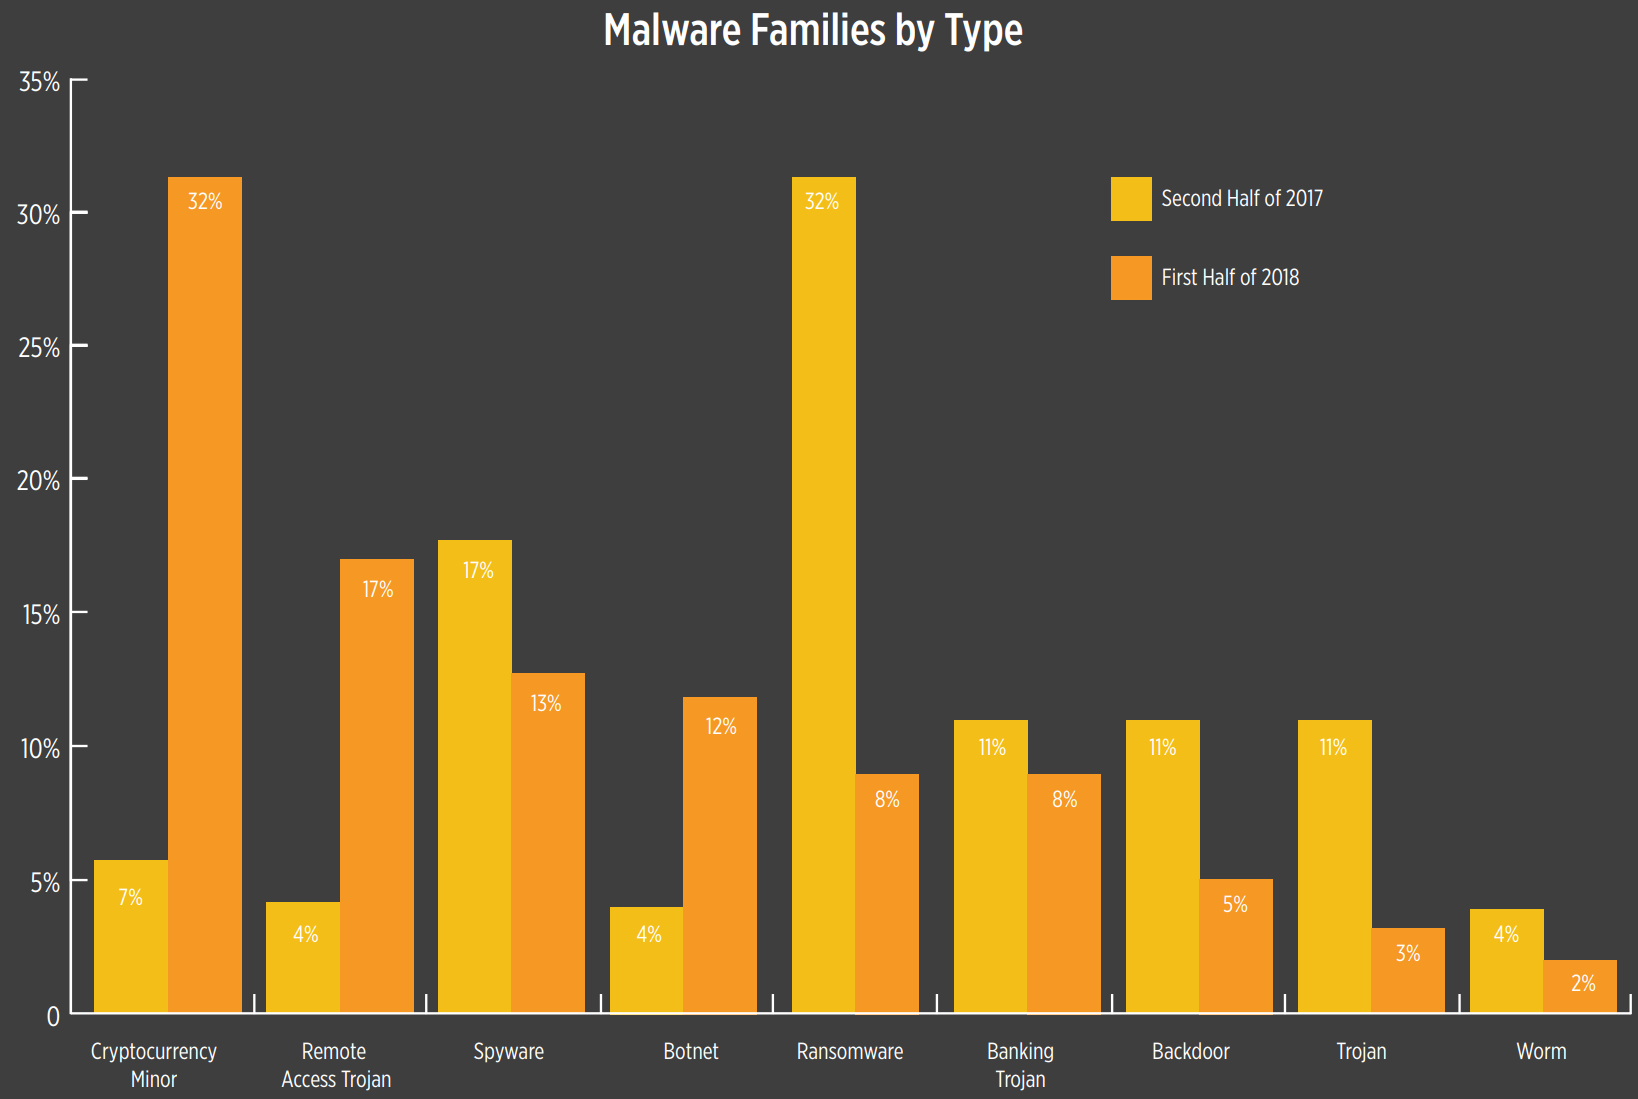
\includegraphics[width=0.8\textwidth]{TopMalwareFamilies.png}
\end{figure}

{\chapter{Proposta di progetto}}
Lo scopo ultimo del progetto è quello di sviluppare un attacco web basato sulla tecnica del \emph{cryptojacking} che operi su GPU e successivamente sviluppare una difesa per attacchi simili.\\
Per il raggiungimento di tale scopo è necessario innanzitutto sviluppare uno script che effettui il \emph{mining} attraverso l'utilizzo della GPU in ambito web. Successivamente creare un sistema che permetta al codice malevolo di raggiungere le vittime attraverso pagine web e testarne l'efficacia in un ambiente simile a quello reale. Una volta sviluppata e testata l'efficienza del sistema di attacco, sarà poi possibile analizzarlo e identificare una modalità di difesa efficiente e, se possibile, utilizzarla per implementare un sistema contro attacchi dello stesso genere.\\
Per il raggiungimento dei due obiettivi principali si è pensato all'utilizzo combinato di librerie che permettono l'interazione con la GPU in ambito web e  tipologie di attacco che permettono l'iniezione di codice malevolo all'interno di applicativi web.\\
Si è quindi preso in considerazione l'utilizzo di librerie come \citetitle{WebGL}, in particolare \citetitle{GPU.js} che, come dimostrato proprio dagli sviluppatori~\citep{banchmarkGPU.js}, computa circa quindici volte più velocemente della sola CPU il caricamento di elementi grafici complessi. Operando in un contesto di grafica tridimensionale, queste implementazioni permettono di effettuare operazioni anche complesse attraverso la GPU dell'utente che visualizza la pagina web dove sono utilizzate. L'idea è quindi quella di sviluppare un \emph{cryptominer} attraverso l'utilizzo di queste librerie e del linguaggio \emph{Javascript}. La scelta di questo linguaggio non è dovuta solo al fatto che è uno dei più utilizzati e supportati all'interno del web \citep{w3techsJavascriptPopularity}, ma anche al fatto che si presta benissimo per l'iniezione di codice malevolo come mostrato da~\citen{owaspxss}.\\
Infatti, per poter raggiungere le vittime ed effettuare l'operazione di \emph{mining} tramite pagine \emph{HTML}, è necessario che lo script creato sia presente nella struttura della pagina visitata dalle vittime. Per fare ciò si potrebbe creare un'applicazione web con il codice malevolo ma questa non sembra essere la soluzione migliore, in quanto, oltre a raggiungere un numero molto limitato di vittime, aumenterebbe il rischio di essere scoperti nel caso si stesse effettuando un attacco reale. Proprio per rendere l'attacco il più veritiero possibile, si è pensato invece di effettuare una simulazione dell'inserimento del codice malevolo all'interno di siti web vulnerabili realmente esistenti, questo sfruttando attacchi di tipo \emph{XSS}.\\
Esistono vari strumenti in grado di analizzare la struttura delle pagine web e di identificare vulnerabilità \emph{XSS}, come ad esempio \citetitlen{XSStrike}, \citetitlen{Traxss} e \citetitlen{XSSer}. Questi sono tutti tool open-source di analisi sviluppati in \emph{Python}, il più interessante è però \citetitle{XSSer}, uno dei tool preinstallati presenti nelle distribuzioni \emph{Linux} atte al \emph{penetration testing}. Si è quindi pensato di utilizzare uno di questi tool per individuare in modo semi-automatico o del tutto automatico le vulnerabilità \emph{XSS} all'interno di siti web. Per l'identificazione dei siti target si utilizzerà una lista pubblica di siti vulnerabili, ad esempio quella fornita da \citen{xssed}. Una volta individuato un buon numero di siti vulnerabili si creerà un ambiente di lavoro dove effettuare i test di \emph{injection}. L'ambiente di test dell'attacco sarà infatti composto da copie dell'intera struttura dei siti vulnerabili identificati riprodotte sulla macchina locale, questo sempre per rendere i test il più veritieri possibile senza realmente effettuare l'attacco verso i siti originali.\\
Una volta testata l'efficacia del sistema di attacco, sarà effettuata un'analisi per individuare una possibile difesa attuabile dagli utenti degli applicativi web. Una possibile soluzione sarebbe quella di sviluppare un'estensione per il browser che individui la presenza di librerie web che utilizzano la GPU e avvertire di ciò l'utente che sta accedendo alla pagina. In questo modo si potrebbe evitare che l'utente acceda al contenuto della pagina sospetta o, che dopo un'attenta verifica, scelga se disabilitare o meno alcune funzionalità della pagina. Questa soluzione potrebbe però non essere efficiente se gli attacchi saranno effettuati con l'aggiunta di tecniche di offuscamento del codice come quella sviluppata da \citen{sharif2008impeding}. In tal caso si potrebbe valutare l'opzione di monitorare le prestazioni dell'hardware per individuare lo svolgimento dell'attacco e bloccarne l'esecuzione. Non saranno effettuate analisi dal punto di vista del \emph{Cross Site Script} in quanto modi per evitare questo tipo di vulnerabilità sono già stati studiati ed analizzati a fondo negli ultimi anni, come è stato fatto proprio da \citen{bisht2008xss}.\\
Lo sviluppo dei sistemi avverrà con l'ausilio di una macchina virtuale, questa scelta non è dovuta tanto ai danni che lo sviluppo potrebbe portare sul sistema, ma al fatto che non si è a conoscenza delle operazioni effettuate dai siti vulnerabili che si andranno a riproporre in copia locale. Inoltre l'utilizzo di una macchina virtuale fornirà un ambiente privo di agenti esterni che possano interferire con l'esecuzione dei sistemi. Il progetto sarà reso pubblico sulla piattaforma \emph{GitHub}\footnote{https://github.com/ZappaBoy/hi-jacket} nel quale saranno presenti lo script del \emph{cryptominer} iniettabile, il sistema semi-automatico o automatico di \emph{injection} tramite \emph{XSS} e se possibile l'implementazione di un metodo di difesa contro attacchi simili a quello sviluppato.

%----------------------------------------------------------------------------------------
%	BIBLIOGRAPHY
%----------------------------------------------------------------------------------------

\printbibliography\
\end{document}
